\section{Modeling incomplete lineage sorting: the multispecies coalescent}
Incomplete lineage sorting is a population-level process.
In a species, at a given time, there are several alleles for a given locus in the genome.
These alleles have their own history, they diverged from each other at various times in the past.
This history can differ from the species history, because several alleles can persist through a speciation event, and because, even without selective effects, the sorting of alleles during a speciation event is random and can result in a tree that differs from the species tree (Fig. \ref{fig1}d).
In all cases, incongruence between the gene tree and the species tree occurs when alleles persist over the course of several speciation events.
When reconstructing a gene tree, one therefore gets the history of the alleles that have been sampled (at best), not the history of the species. 

In 2003, Rannala and Yang proposed a powerful way to model the sorting of alleles along a phylogeny of several species \citep{Rannala2003}, the multispecies coalescent (Fig. \ref{fig2}).
This model is at the origin of most model-based approaches to reconstruct gene and species trees \citep{Edwards2007,Heled2010}.
The multispecies coalescent models the evolution of a population of alleles along a species tree.
Along the species tree, it allows different branch lengths, in units of time, and also allows different effective population sizes.
Computing the probability of a gene tree given a species tree and other parameters is quite easy.
Basically it works by cutting the gene tree into independent species-specific subtrees, computing probabilities for each of those subtrees, and combining them all at the end to get the probability of the gene tree according to the multispecies coalescent, given the current parameter values.
Cutting the gene tree into species-specific subtrees is quite easy, because we can use the dates of speciation events to identify parts of the gene trees that are before and after speciation events. 
The resulting subtrees are represented with the grey boxes in Fig. \ref{fig2}.
In this figure, each subtree corresponds to one particular population, either extant or ancestral.
Inside each subtree, given its length, the effective population size, and dates of coalescence (divergences of alleles), the coalescent model provides simple formulas for computing the probability of the gene subtree given other parameters.
Because we consider that these subtree probabilities are all independent of one another, they are then multiplied to get the gene tree probability given current parameter values.
 
Two parameters associated to branches of the species tree have a direct impact on the expected amount of gene tree-species tree incongruence:
\begin{itemize}
\item \textbf{Time between speciations.} The more a branch length increases, the more the pool of alleles is expected to change.
Alleles are therefore less likely to persist for several speciation events if the branches between these speciation events are long.
\item \textbf{Effective population size between speciations.} In populations with small effective population sizes, chance events can cause large shifts in allele frequencies, and possibly disappearance of alleles. 
In large populations, because an allele is likely carried by a large number of individuals, its disappearance is less likely, the population of alleles is more stable.
Alleles are therefore less likely to persist for several speciation events if the branches between these speciation events are characterized by small effective population sizes.
\end{itemize}
Overall, larger amounts of gene tree-species tree incongruence are expected in phylogenies characterized by short branches with large population sizes. 
A corollary of that is that larger amounts of gene tree-gene tree incongruence are expected as well. 
To measure the susceptibility of species phylogenies to generate incomplete lineage sorting, the concept of \emph{coalescent time units} has been introduced.
Coalescent time units are obtained when branch length $\lambda$, in number of generations, is divided by effective population size $N_e$.
As a consequence, in a species tree whose branches are expressed in coalescent time units, a branch length of $1~coalescent~time~unit $ means a branch length of $N_e~generations$. 
Once branch lengths on the species tree are measured in coalescent time units, it becomes easy to spot species trees that generate a lot of incongruence: those are short trees.

\begin{figure}[h!]
\centering
\fbox{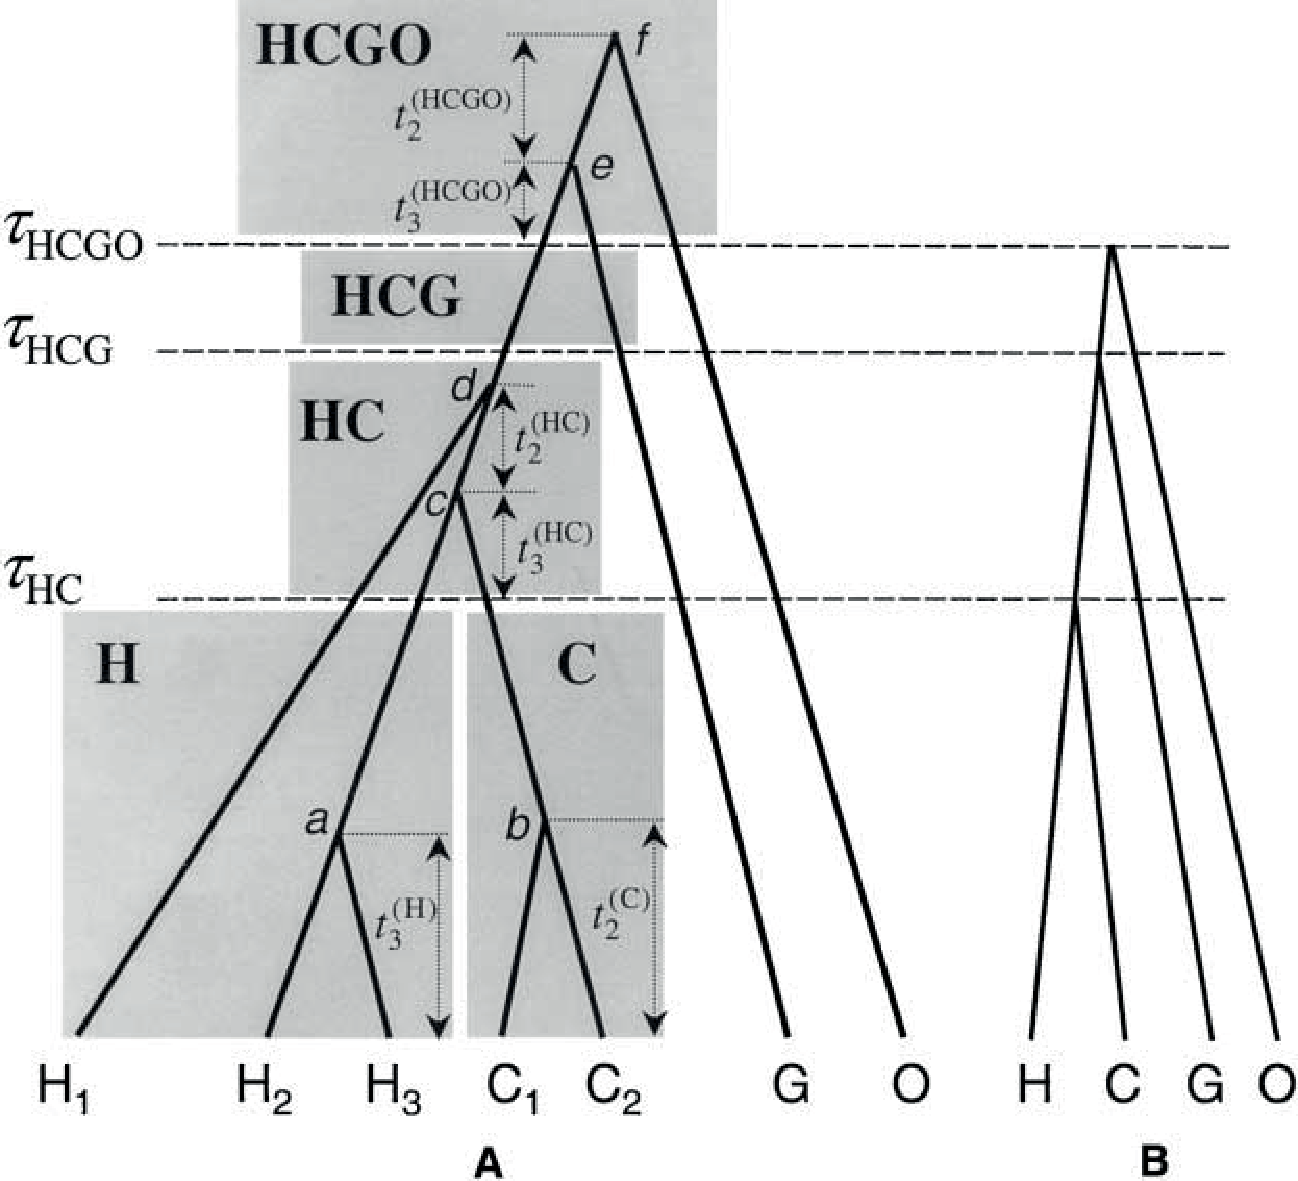
\includegraphics[width=5.8in,angle=0]{\ResourcePath figures/RannalaYang.pdf}}
\caption{\small The multispecies coalescent. A) A gene tree, including 3 human alleles, 2 Chimp alleles, one Gorilla allele, and one Orang-outan allele. $\tau$ parameters are speciation times, $t$ parameters are divergence time in the gene tree, the grey squares represent the ancestral populations, with their respeciive sizes.  B) The corresponding species tree. In this model, the speciation times define minimal boundaries for allele divergence times. [Replicated from Fig.~1 in \citet{Rannala2003}.]}
\label{fig2}
\end{figure}

\vspace{20mm}

{\begin{framed}
\begin{center}
The exercises assume you have a working installation of RevBayes.
In this introductory tutorial, we will apply the multispecies coalescent model to 10 gene alignments from 23 primate species.
We will specify the multispecies coalescent, with different effective population sizes for each branch of the species tree.
We will assume that:
\begin{itemize}
\item The species tree is drawn from a constant birth-death process.
\item Along the branches of the species tree, a multispecies coalescent process generates gene trees. Different effective population sizes are assigned to each branch of the species tree.
\item Along each gene tree, gene sequences are evolved according to an HKY modeland a strict global clock. To save computing time, we do not use gamma distributed rate variation among sites.
\item Here, we run an MCMC on this model, using data from 10 genes in 23 mammalian species.
\end{itemize}
Scripts are all placed in {\footnotesize \emph{$tutorials/RB\_MultispeciesCoalescent\_Tutorial/scripts/$}}. 
\end{center}
\end{framed}}
\vspace{5mm}

\begin{enumerate}
\item Open RevBayes
\item Let's load all 10 gene alignments.

{\tt \begin{snugshade*}
\begin{lstlisting}

### Read in sequence data for all genes

locus_names = ["COIII", "FGA", "GHRmeredith", "lrpprc_169", "npas3", "sim1", "tex2", "ttr", "zfy", "zic3"]

num_loci = locus_names.size()

# read in each data matrix separately
for ( i in 1:num_loci ) {
    data[i] <- readDiscreteCharacterData("data/" + locus_names[i] + ".fasta")
}
# alternatively we could have read in from data/merged.nex too (although that contains the empty sequences ...)

# Get some useful variables from a species tree.
# We need these variables later on, but we will not use the species tree as starting value.
primate_tree = readTrees("data/primates.tree")[1]
n_species <- primate_tree.ntips()
taxa <- primate_tree.taxa()
n_branches <- 2 * n_species - 1 # number of branches in a rooted tree

# set my move index
mi = 0

\end{lstlisting}
\end{snugshade*}}

\item We specify a constant-rate birth-death process as our prior on the species tree. 
The birth-death process has a speciation and extinction rate as its parameters. 
We use here a transformation and specify priors on the speciation rate and relative extinction rate.
Additionally, we calibrate the tree by assuming that the crown age of primates is around 75 MYA.
Thus, we specify a normal distribution with mean 75 and standard deviation 2.5 as the prior on the root age.
Since the root age can only be a positive real number we truncate the normal distribution at 0.

{\tt \begin{snugshade*}
\begin{lstlisting}

# Specify a prior on the diversification and turnover rate
speciation ~ dnGamma(2,2)
relativeExtinction ~ dnBeta(1,1)

# now transform the diversification and turnover rates into speciation and extinction rates
extinction := speciation * relativeExtinction

# specify a prior on the root age (our informed guess is about 75-80 mya)
root ~ dnNormal(mean=75,sd=2.5,min=0.0, max=Inf)

sampling_fraction <- 23 / 450 # 23 out of the ~ 450 primate species

# create some moves that change the stochastic variables
# all moves are sliding and scaling proposals
moves[++mi] = mvSlideBactrian(speciation,tune=true,weight=2)
moves[++mi] = mvSlideBactrian(relativeExtinction,tune=true,weight=2)
moves[++mi] = mvScaleBactrian(speciation,lambda=1,tune=true,weight=2)
moves[++mi] = mvScaleBactrian(relativeExtinction,lambda=1,tune=true,weight=2)


# construct a variable for the tree drawn from a birth death process
psi ~ dnBDP(lambda=speciation, mu=extinction, rootAge=root, rho=sampling_fraction, taxa=taxa )

\end{lstlisting}
\end{snugshade*}}

\item Mixing in the multispecies coalescent model is particularly challenging. 
Although, in principle and assuming our MCMC is working as intended, after an infinite amount of time we would converge to a correct estimate of the posterior distribution over the species tree, gene trees and other parameters, it is advisable to start from reasonable starting values for the species tree and the gene trees.
In our case, we have already reconstructed candidate gene trees using RevBayes.
These gene trees have been produced using the scripts: \\ {\footnotesize \emph{$tutorials/RB\_MultispeciesCoalescent\_Tutorial/scripts/mcmc\_GeneTree.Rev$}} and \\ {\footnotesize \emph{$tutorials/RB\_MultispeciesCoalescent\_Tutorial/construct\_all\_GeneTrees.sh$}}).
They have been placed in the folder {\footnotesize \emph{$tutorials/RB\_MultispeciesCoalescent\_Tutorial/output\_GeneTrees$}}, and Maximum A Posteriori (MAP) trees have been constructed.
These MAP trees will provide good starting gene trees, and will also be used to generate a starting species tree using a function that computes a maximum tree \citep{Edwards2007}.
The maximum tree "is the tree with the largest possible speciation times in the space of species trees restricted by available gene trees" \citep{Liu2010}.
Conveniently, tip names in the gene trees correspond to the species names: we can thus use the maximum tree function on these trees without worrying about potential name inconsistencies.

{\tt \begin{snugshade*}
\begin{lstlisting}

# read in each gene tree separately
j=1
for ( i in 1:num_loci ) {
    gene_trees[i] <- readTrees("output_GeneTrees/" + locus_names[i] + "_MAP.tree")[1]
    print("Gene tree "+i+ " has "+ gene_trees[i].ntips() + " tips.")
}

# We set the species tree to a good starting value.
# This good starting value is obtained from the Maximum Tree method (Liu, 2006).
# The same method is used in BEST to obtain a good starting species tree.
recTree <- maximumTree(gene_trees)
psi.setValue(recTree)
root.setValue(recTree.rootAge())

write("\t\tProposed starting species tree: ")
write( psi)
write("\t\tWith root age: " + root)

\end{lstlisting}
\end{snugshade*}}

\item Now that we have a species tree, we can specify the prior on the gene trees by using a multispecies coalescent process.
First, we need to load in a map of the individual names to the species names.
This map ensures we can associate the individuals to the species they belong to.
Have a look in one of these files, for example \textit{primates\_COIII\_species\_map.txt}.
We will assume that each branch of the species tree, which represents a population, has its own population size.
Thus, our prior is that each population size per branch is identically distributed from an exponential distribution with rate 0.1 (giving an expectation of 10 and thus a relatively flat prior distribution).
Note that we use fixed population sizes for the terminal branches because we have only a single individual per species and thus have no information about its population size.
One could use other models for the population sizes.
For example one could assume that all branches have the same population size.
Once the gene trees have been declared, we set their value to the MAP trees that we have read previously.

{\tt \begin{snugshade*}
\begin{lstlisting}

# We assume independent effective population size parameters for each branch of the species tree.
for (i in 1:n_species) {
  Ne[i] <- 10.0
}
for (i in (n_species+1):n_branches) {
  Ne[i] ~ dnExponential(0.01)
  moves[++mi] = mvScale(Ne[i],lambda=.1,tune=true,3.0)
  moves[++mi] = mvSlide(Ne[i],tune=true,2.0)

}

# We could also assume a single effective population size for the entire species tree.
#Ne ~ dnGamma(shape=1.0,rate=1.0)
#moves[++mi] = mvScale(Ne,1,true,1.0)

for (i in 1:num_loci) {

   # We need to read in files providing the link between gene names and species names
   taxon_map = readTaxonData("data/species_maps/primates_" + locus_names[i] + "_species_map.txt")

   # The gene tree from the multispecies coalescent process
   # Note that if Ne had been a vector of effective population sizes,
   # allowing 1 parameter per branch of the species tree, the same line would work.
   geneTree[i] ~ dnMultiSpeciesCoalescent(speciesTree=psi, Ne=Ne, taxa=taxon_map)
   # We set a good starting value
   geneTree[i].setValue(gene_trees[i])

}

\end{lstlisting}
\end{snugshade*}}

\item Although we have defined both the species tree and the gene trees, we have not set up the moves that we use to sample them.
We will use simple tree moves, that deal with a single tree at a time, and joing species tree-gene tree moves.
Those latter moves are important because they explicitly take into account the interdependency between the species tree and the gene trees.
These moves are first declared with the species tree as main argument. 
Then, each gene tree is added to the moves.


{\tt \begin{snugshade*}
\begin{lstlisting}

## General tree moves used on the species tree
moves[++mi] = mvNarrow(psi, weight=5.0)
moves[++mi] = mvNNI(psi, weight=1.0)
moves[++mi] = mvFNPR(psi, weight=3.0)
moves[++mi] = mvGPR(psi, weight=3.0)
moves[++mi] = mvSubtreeScale(psi, weight=3.0)
moves[++mi] = mvNodeTimeSlideUniform(psi, weight=5.0)

## Joint species tree/gene tree moves
move_species_narrow_exchange = mvSpeciesNarrow( speciesTree=psi, weight=20 )
move_species_subtree_scale_beta = mvSpeciesSubtreeScaleBeta(psi, weight=5)
move_species_subtree_scale = mvSpeciesSubtreeScale(psi, weight=5)

## Moves that alter gene trees
for (i in 1:num_loci) {

    # moves on each gene tree
    moves[++mi] = mvNNI(geneTree[i], 5.0)
    moves[++mi] = mvNarrow(geneTree[i], 5.0)
    moves[++mi] = mvFNPR(geneTree[i], 3.0)
    moves[++mi] = mvGPR(geneTree[i], 2.0)
    moves[++mi] = mvSubtreeScale(geneTree[i], 5.0)
    moves[++mi] = mvTreeScale(geneTree[i], 1.0, true, 3.0)
    moves[++mi] = mvNodeTimeSlideUniform(geneTree[i], 20.0)

    # Associating the joint species tree/gene tree moves to each gene tree
    move_species_narrow_exchange.addGeneTreeVariable( geneTree[i] )
    move_species_subtree_scale_beta.addGeneTreeVariable( geneTree[i] )
    move_species_subtree_scale.addGeneTreeVariable( geneTree[i] )

}

## We must not forget to include the joint moves into the vector of moves!
moves[++mi] = move_species_narrow_exchange
moves[++mi] = move_species_subtree_scale_beta
moves[++mi] = move_species_subtree_scale




\end{lstlisting}
\end{snugshade*}}


\item Now we have gene trees, complete with branch lengths, and the moves operating on them. 
The next element we need is a clock rate which transforms/scales the branch times into branch lengths that represent the expected number of substitutions.
Here we will assume for simplicity that every gene evolves under a global strict clock but has its own independent clock rate.
We can later look into the estimate to see how much the clock rate estimates actually differ across genes.
One could also choose to use a relaxed clock model instead of a strict clock.

{\tt \begin{snugshade*}
\begin{lstlisting}

for ( i in 1:num_loci ) {
   clock_rate[i] ~ dnExponential(1.0)
   moves[++mi] = mvScale(clock_rate[i], weight=2.0)
   moves[++mi] = mvSlide(clock_rate[i], weight=3.0)
}
\end{lstlisting}
\end{snugshade*}}

\item Next we need our model for the substitution process. 
Hence, we just need to define the substitution matrix. 
We use a single HKY matrix that will apply to all sites per gene.
Additionally, we assume that sites all evolve according to the same rate, to save computing time.
{\tt \begin{snugshade*}
\begin{lstlisting}
for ( i in 1:num_loci ) {

    #### specify the HKY substitution model applied uniformly to all sites ###
    kappa[i] ~ dnLognormal(0,1)
    moves[++mi] = mvScale(kappa[i],weight=1.0)
    moves[++mi] = mvSlide(kappa[i], weight=1.0)

    pi_prior[i] <- v(1,1,1,1)
    pi[i] ~ dnDirichlet(pi_prior[i])
    moves[++mi] = mvSimplexElementScale(pi[i],weight=2.0)

    #### create a deterministic variable for the rate matrix ####
    Q[i] := fnHKY(kappa[i],pi[i])

}

\end{lstlisting}
\end{snugshade*}}


\item Finally, we can create our distribution for character evolution.
We will use the common \cl{PhyloCTMC} distribution, which is a continuous time Markov process along a phylogenetic tree.
We create a \cl{seq} variable and attach/clamp each gene to one of the \cl{seq} variables.
{\tt \begin{snugshade*}
\begin{lstlisting}
for ( i in 1:num_loci ) {
    # the sequence evolution model
    seq[i] ~ dnPhyloCTMC(tree=geneTree[i], Q=Q[i], branchRates=clock_rate[i], type="DNA")

    # attach the data
    seq[i].clamp(data[i])
}
\end{lstlisting}
\end{snugshade*}}


\item Now we have defined all the bricks of the model, and create our model object from it.
{\tt \begin{snugshade*}
\begin{lstlisting}
# We get a handle on our model.
# We can use any node of our model as a handle, here we choose to use the topology.
mymodel = model(psi)
\end{lstlisting}
\end{snugshade*}}


\item Finally, we need to perform inference under the model, using the data.
For clarity, we put the results in an output folder, and the gene trees will be further included within a folder of their own.
{\tt \begin{snugshade*}
\begin{lstlisting}
output_folder = "output_MSC/"

# Monitors to check the progression of the program
monitors[1] = mnScreen(printgen=100, psi)
monitors[2] = mnModel(filename=output_folder+"posterior_MSC_primates.log",printgen=10, separator = TAB)
monitors[3] = mnFile(filename=output_folder+"posterior_MSC_primates.trees",printgen=10, separator = TAB, psi)
for ( i in 1:num_loci ) {
    # We add a monitor for each gene tree
    monitors[i+3] = mnFile(filename=output_folder+"geneTrees/posterior_" + locus_names[i] + ".trees",printgen=10, separator = TAB, geneTree[i])
}

# Here we use a plain MCMC. You could also set nruns=2 for an analysis with 2 replicates.
# or use mcmcmc with heated chains.
mymcmc = mcmc(mymodel, monitors, moves, nruns=1)

# Ideally one would run more MCMC samples.
# In the interest of time it may be worth running the analysis under the prior.
mymcmc.burnin(generations=1000,tuningInterval=50)#, underPrior=true)
mymcmc.run(generations=3000)#, underPrior=true)


mymcmc.operatorSummary()


\end{lstlisting}
\end{snugshade*}}

\item Now we can perform some post-run analyses, for instance to obtain and save the MAP species tree.
{\tt \begin{snugshade*}
\begin{lstlisting}

# Now, we will analyze the tree output.
# Let us start by reading in the tree trace
treetrace = readTreeTrace(output_folder+"posterior_MSC_primates.trees", treetype="clock")
# and get the summary of the tree trace
treetrace.summarize()

mapTree(treetrace,output_folder+"posterior_MSC_primates_MAP.tree")

\end{lstlisting}
\end{snugshade*}}

%\end{itemize}
\end{enumerate}



\section{Things to think about}
%How did the different methods perform? 
%Did you expect to see these differences?
%It has been shown that the concatenation approach could be inconsistent under some conditions of population size and of divergence times \citep{Degnan2006}. 
%Do you find that concatenation performs worse that its competitors?
%Which models seem to "mix" better?
%In particular, does the full multispecies coalescent mix well?
%Why can we expect this model in particular would have difficulties mixing?
Do you find that the full multispecies coalescent mixes well?\\
Is the mixing markedly different when the model is run under the prior?\\
What is the impact of species tree moves on the mixing?\\
Given the acceptance ratios of some of the moves, would you be tempted to change the frequency at which they are tried? If so how?\\
What other improvements could be made to the script?


\bibliographystyle{sysbio}
\bibliography{\GlobalResourcePath refs}

